\section{Diagramas BPMN}

A modelação do processo ETL é complementada pela criação de diagramas BPMN que permitem representar de forma clara e sistemática o fluxo de atividades envolvidas na preparação dos dados que irão alimentar o data warehouse. Estes diagramas facilitam a compreensão das várias fases do processo, permitindo identificar dependências e contribuem para a deteção de possíveis pontos de melhoria na execução das tarefas.

Existem três níveis de diagramas BPMN que representam a aplicação do processo ETL, sendo eles: nível do processo; nível padrão e nível da tarefa. Sendo que, no âmbito deste projeto, não foi necessário a especificação dos diagramas ao nível da tarefa, como também não foram descritos de forma individual todos os processos ao nível padrão, visto que são todos bastante semelhantes entre si 

\subsection{Visão Global do Processo}

Esta subsecção irá acolher o diagrama BPMN ao nível do processo. O objetivo deste nível é oferecer uma visão abrangente das principais etapas que compõem o fluxo do processo ETL, desde a obtenção das fontes de dados até ao carregamento final no data warehouse. A representação global permitirá compreender a articulação entre as atividades nucleares do sistema, bem como o percurso lógico seguido pelos dados ao longo de todo o ciclo de tratamento.

\begin{figure}[h!]
	\centering
	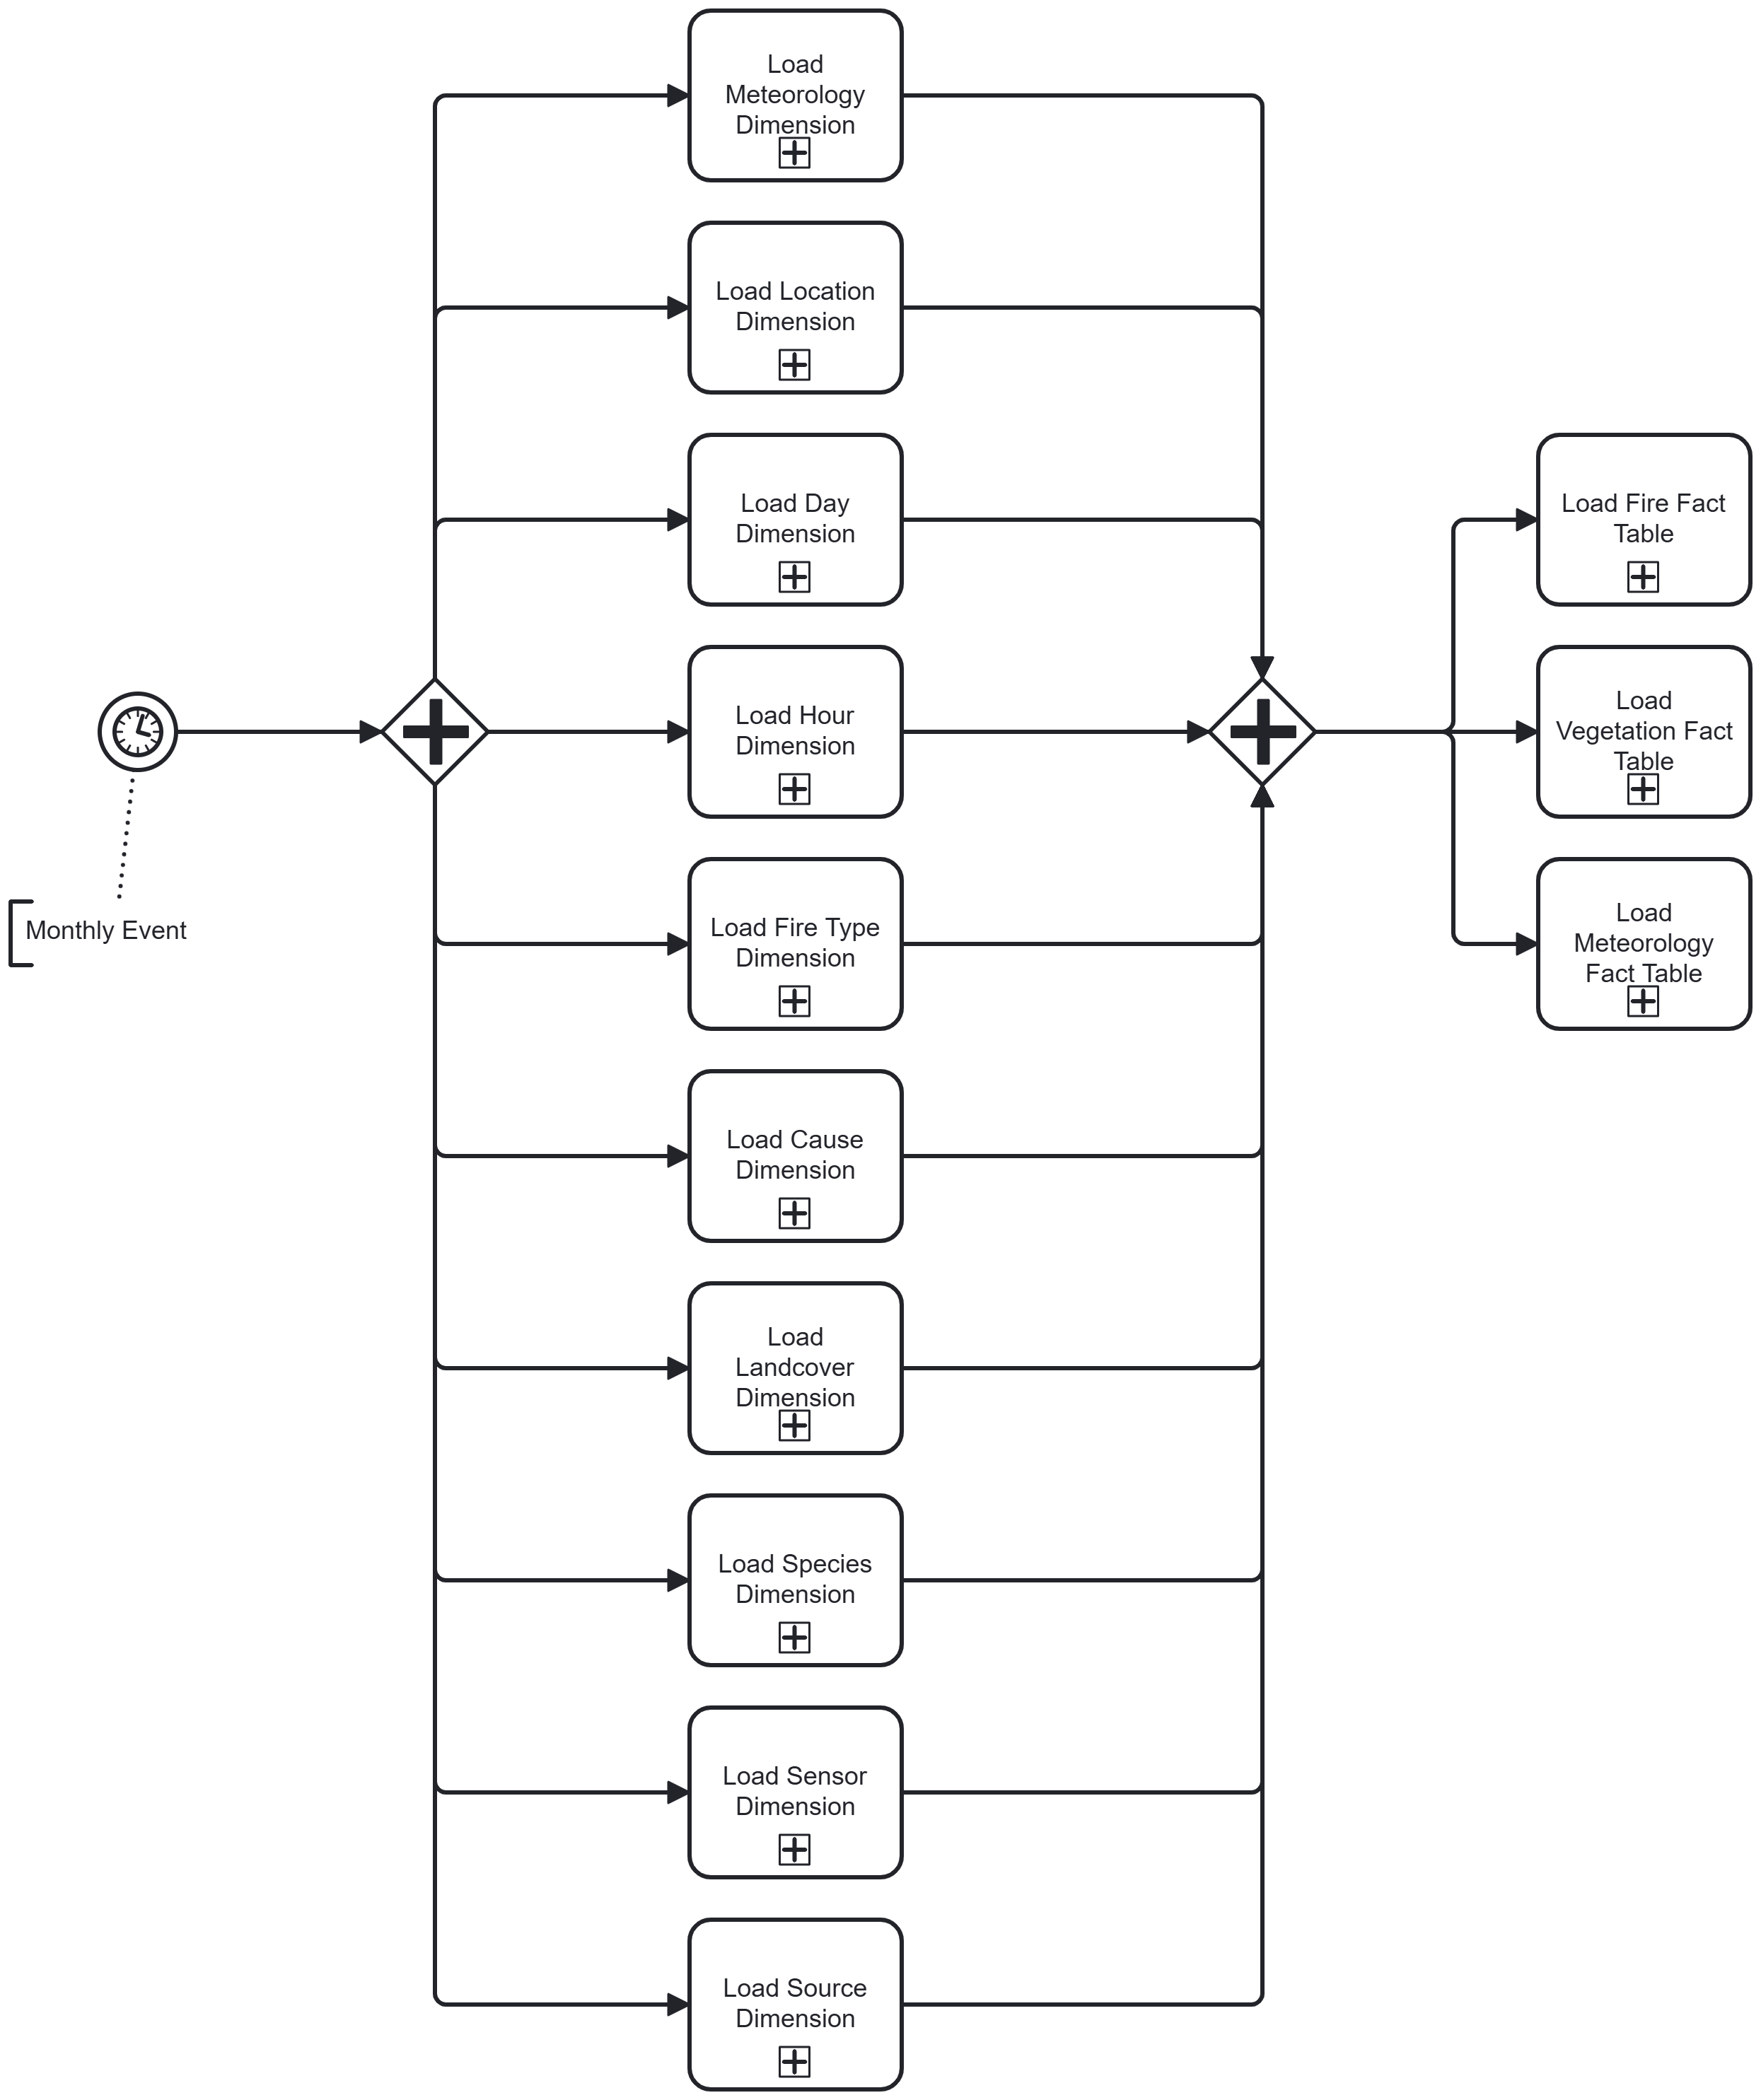
\includegraphics[width=1\linewidth]{imagens/BPMN_Processo}
	\caption{Diagrama BPMN ao nível do processo}
	\label{fig:bpmnprocesso}
\end{figure}



\subsection{Detalhe de Atividades Específicas}

Algumas partes do processo ETL serão representadas por diagramas BPMN ao nível padrão. Estes diagramas permitem aprofundar tarefas que exigem uma descrição mais granular, como procedimentos de validação, mecanismos de controlo de qualidade ou etapas específicas de transformação e enriquecimento dos dados provenientes das diferentes fontes.

\begin{figure}[h]
	\centering
	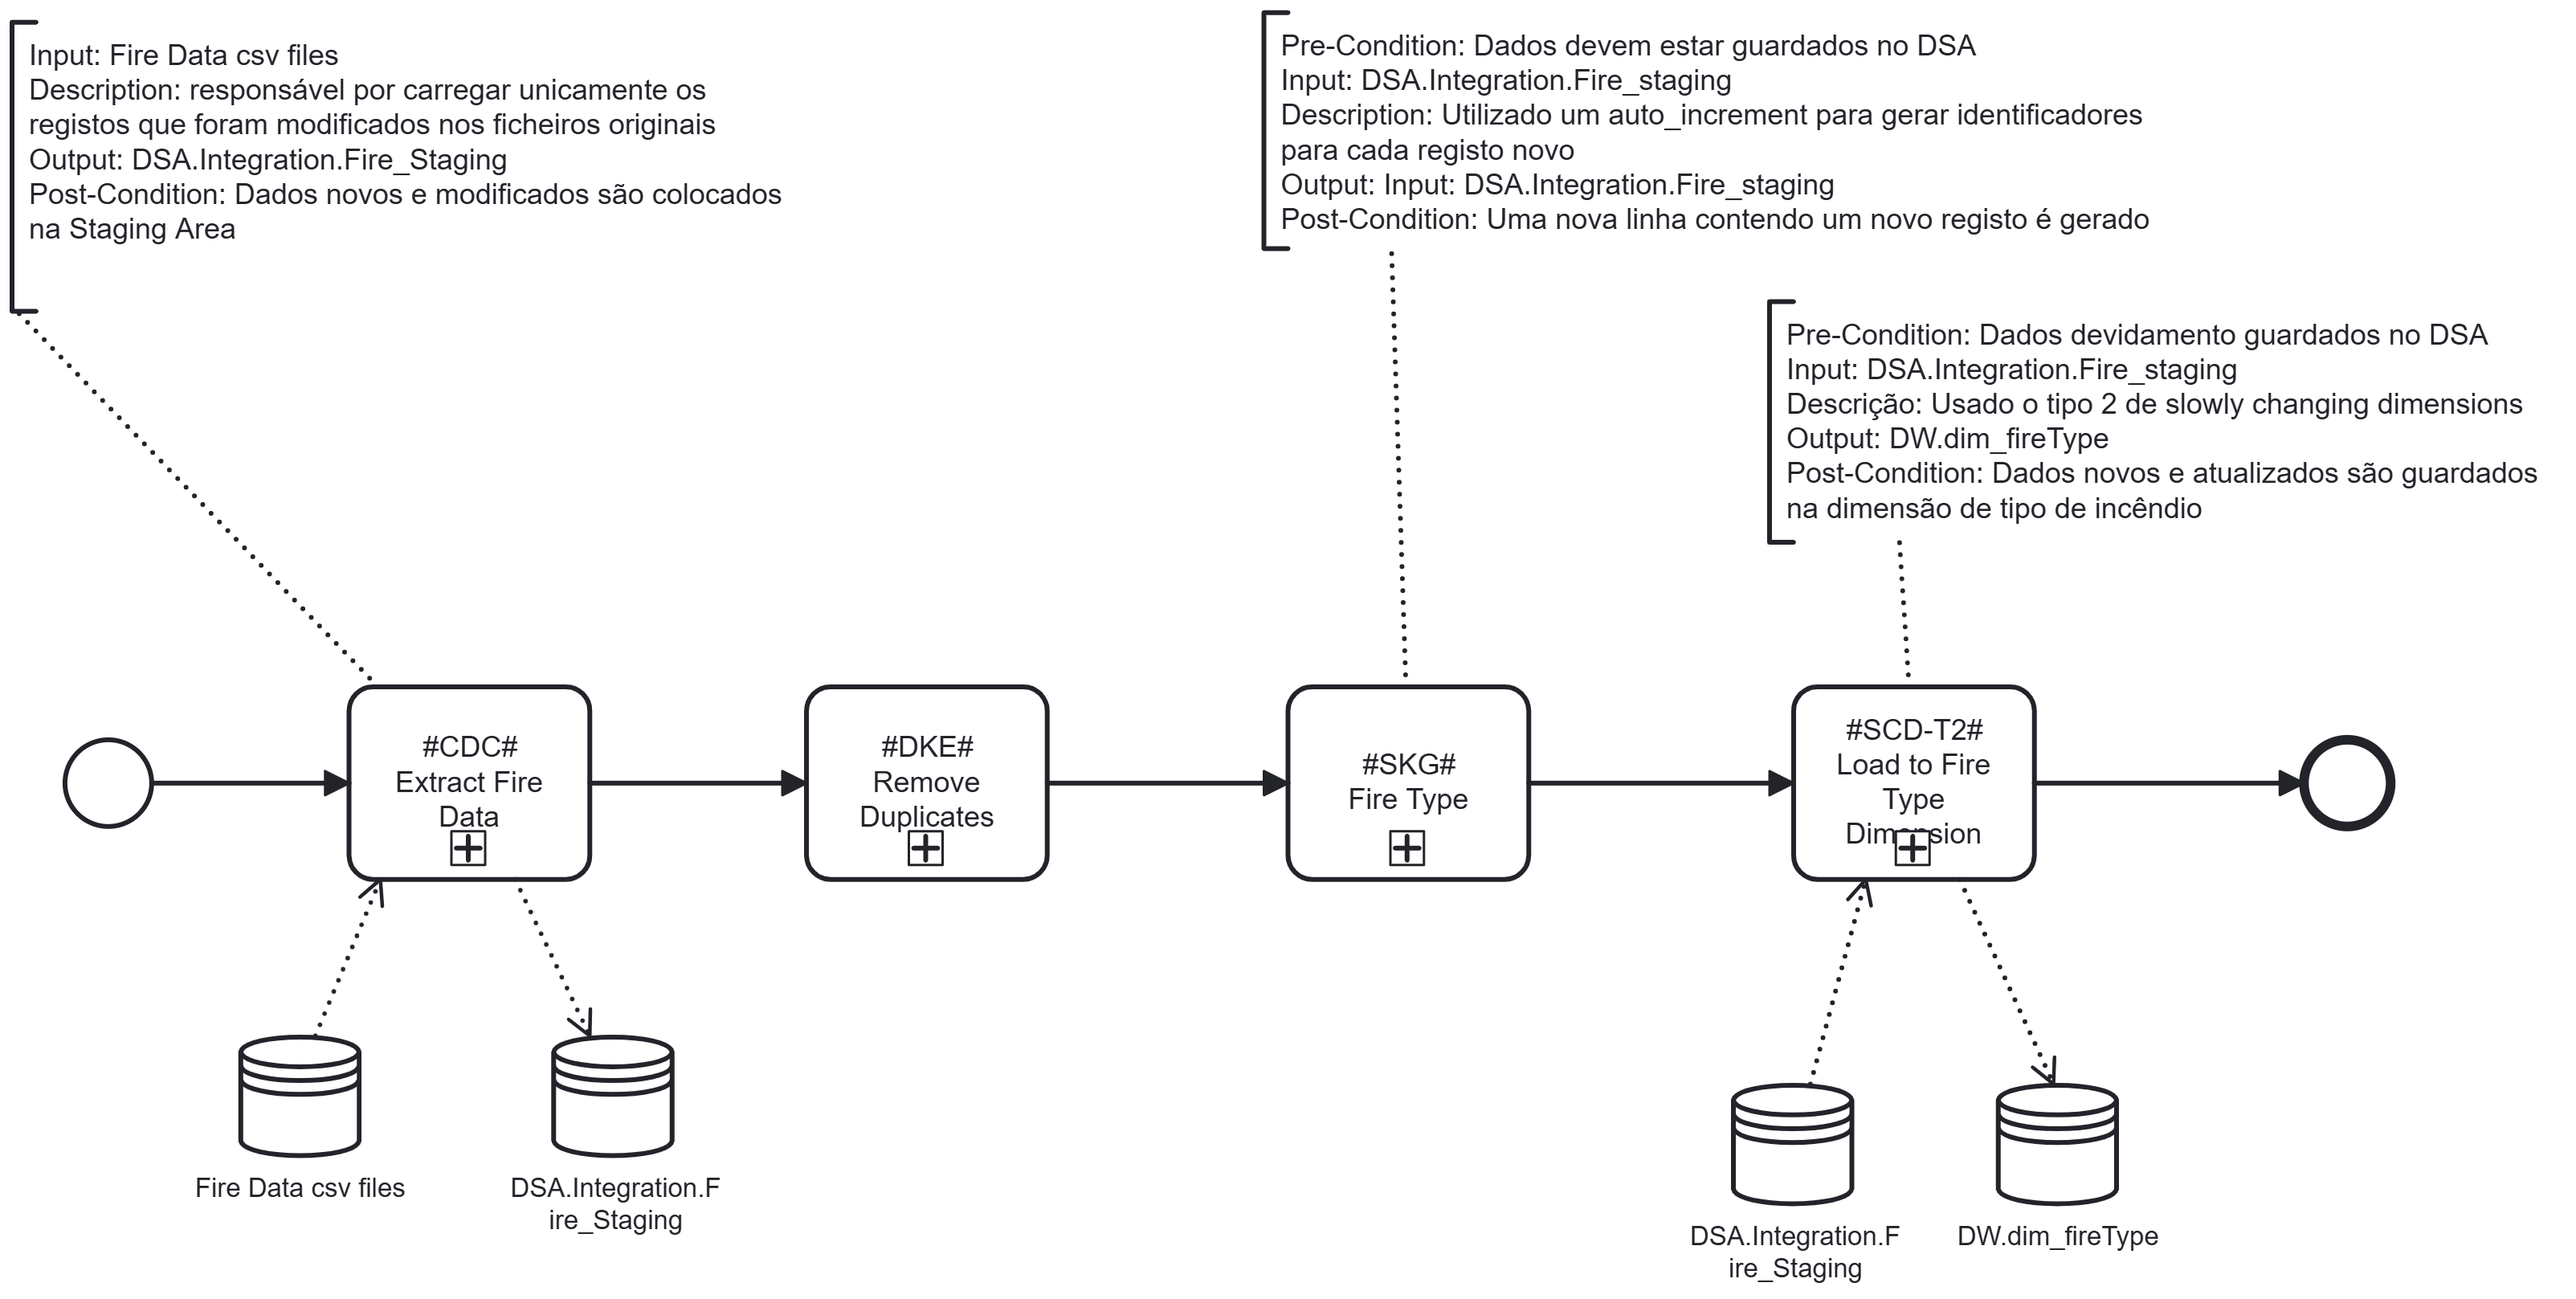
\includegraphics[width=1\linewidth]{imagens/BPMN_Processo_Load_Fire_Type_Dimension}
	\caption{Diagrama BPMN nível padrão para a dimensão tipo de incêndio}
	\label{fig:bpmnprocessoloadfiretypedimension}
\end{figure}

\begin{figure}[h]
	\centering
	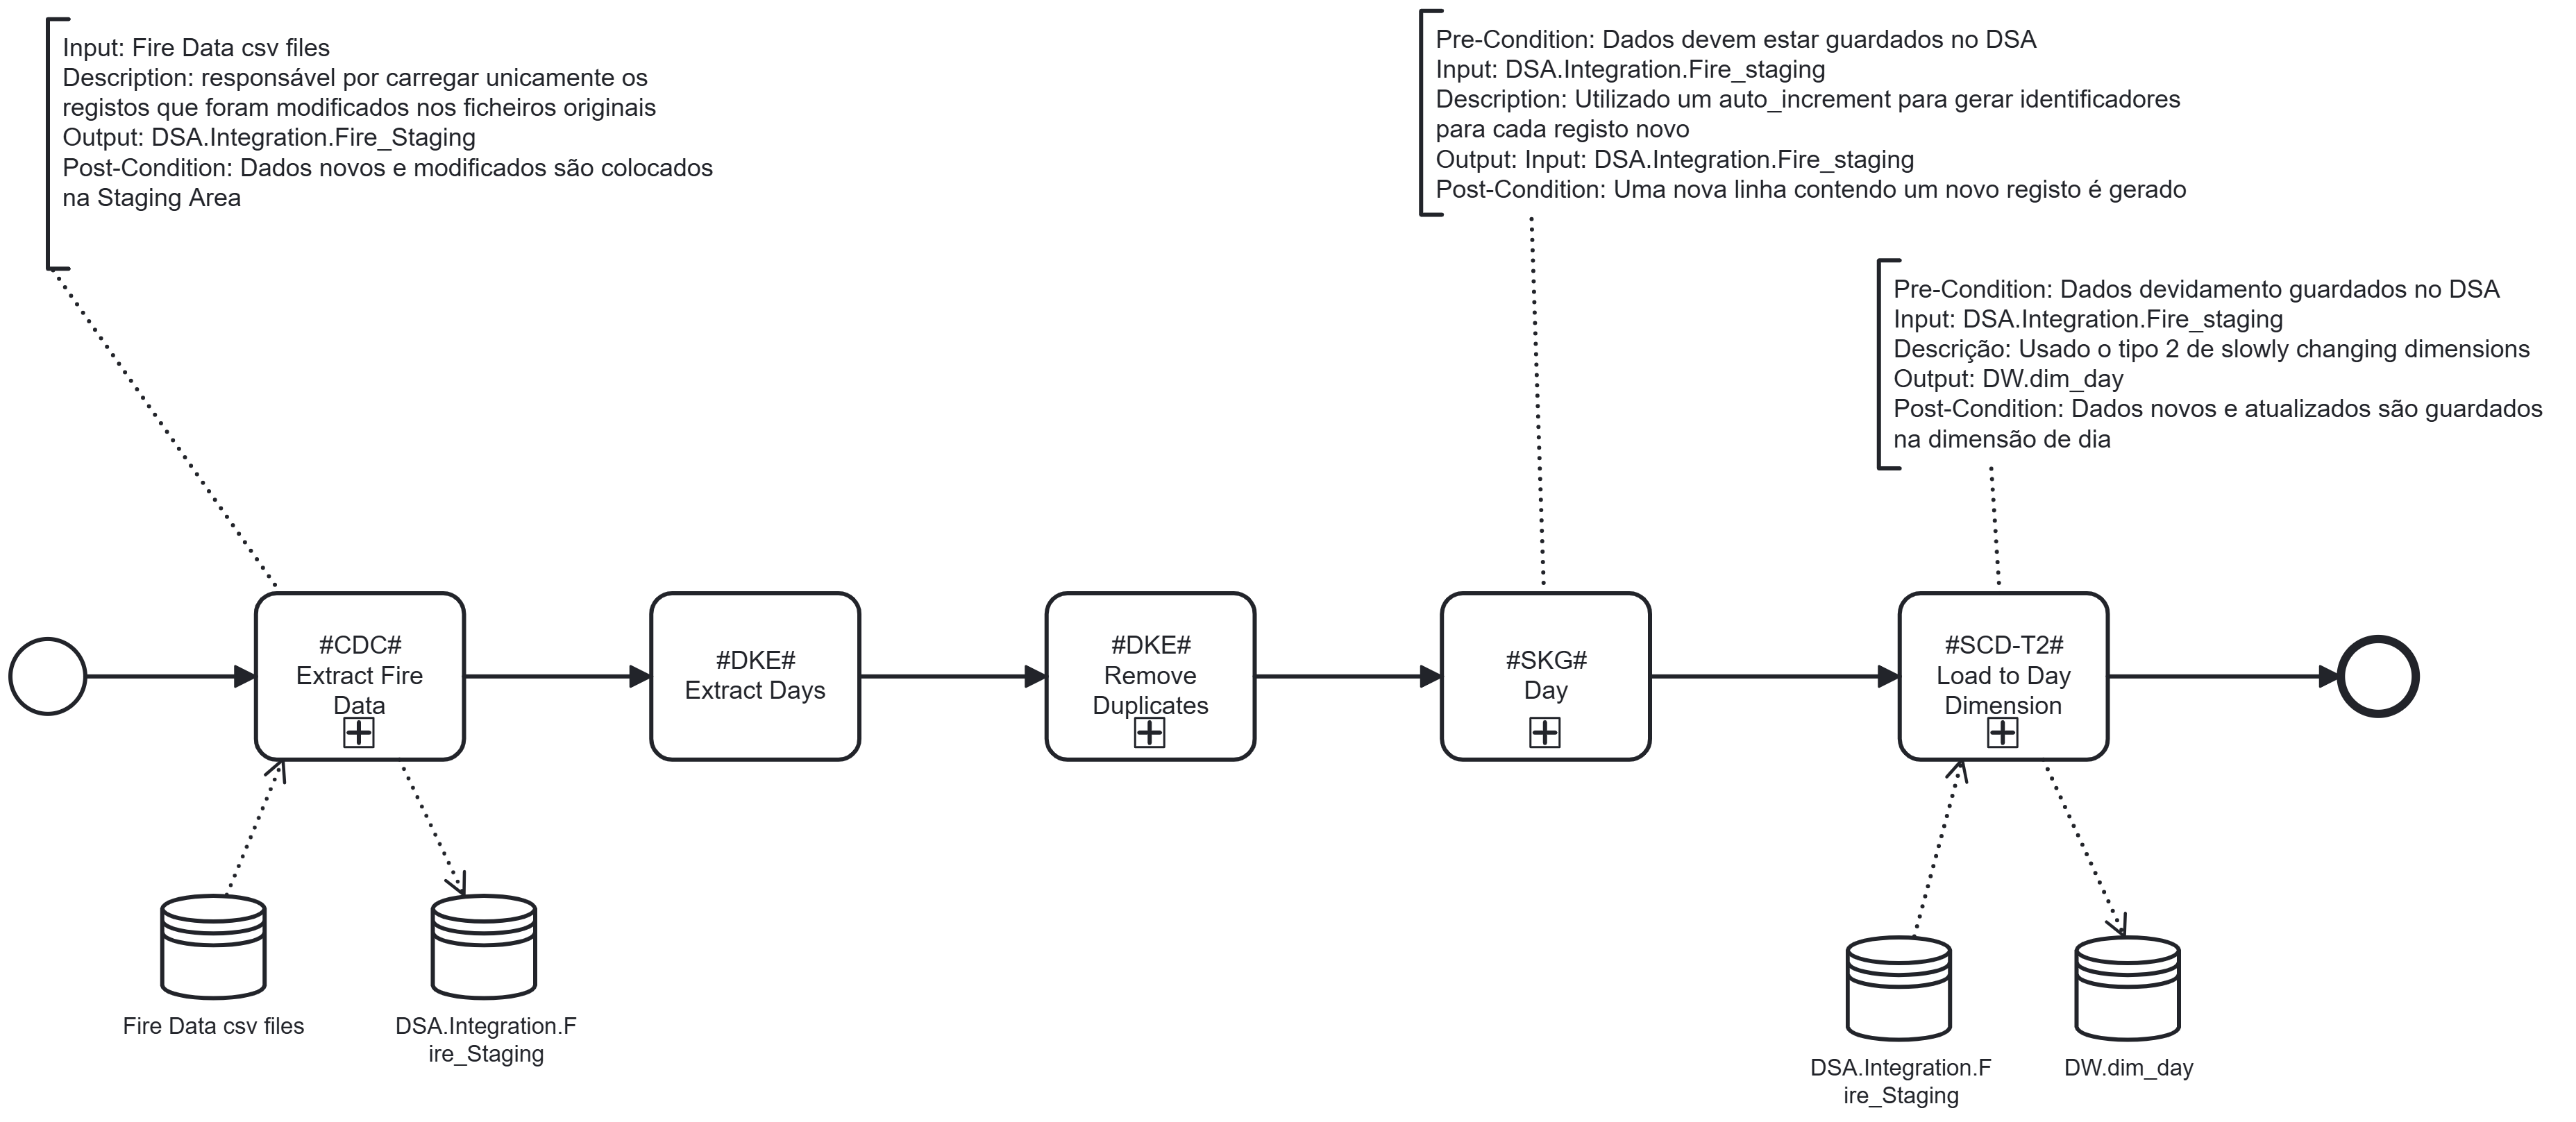
\includegraphics[width=1\linewidth]{imagens/BPMN_Processo_Load_Day_Dimension}
	\caption{Diagrama BPMN nível padrão para dimensão dia}
	\label{fig:bpmnprocessoloaddaydimension}
\end{figure}

\begin{figure}[h]
	\centering
	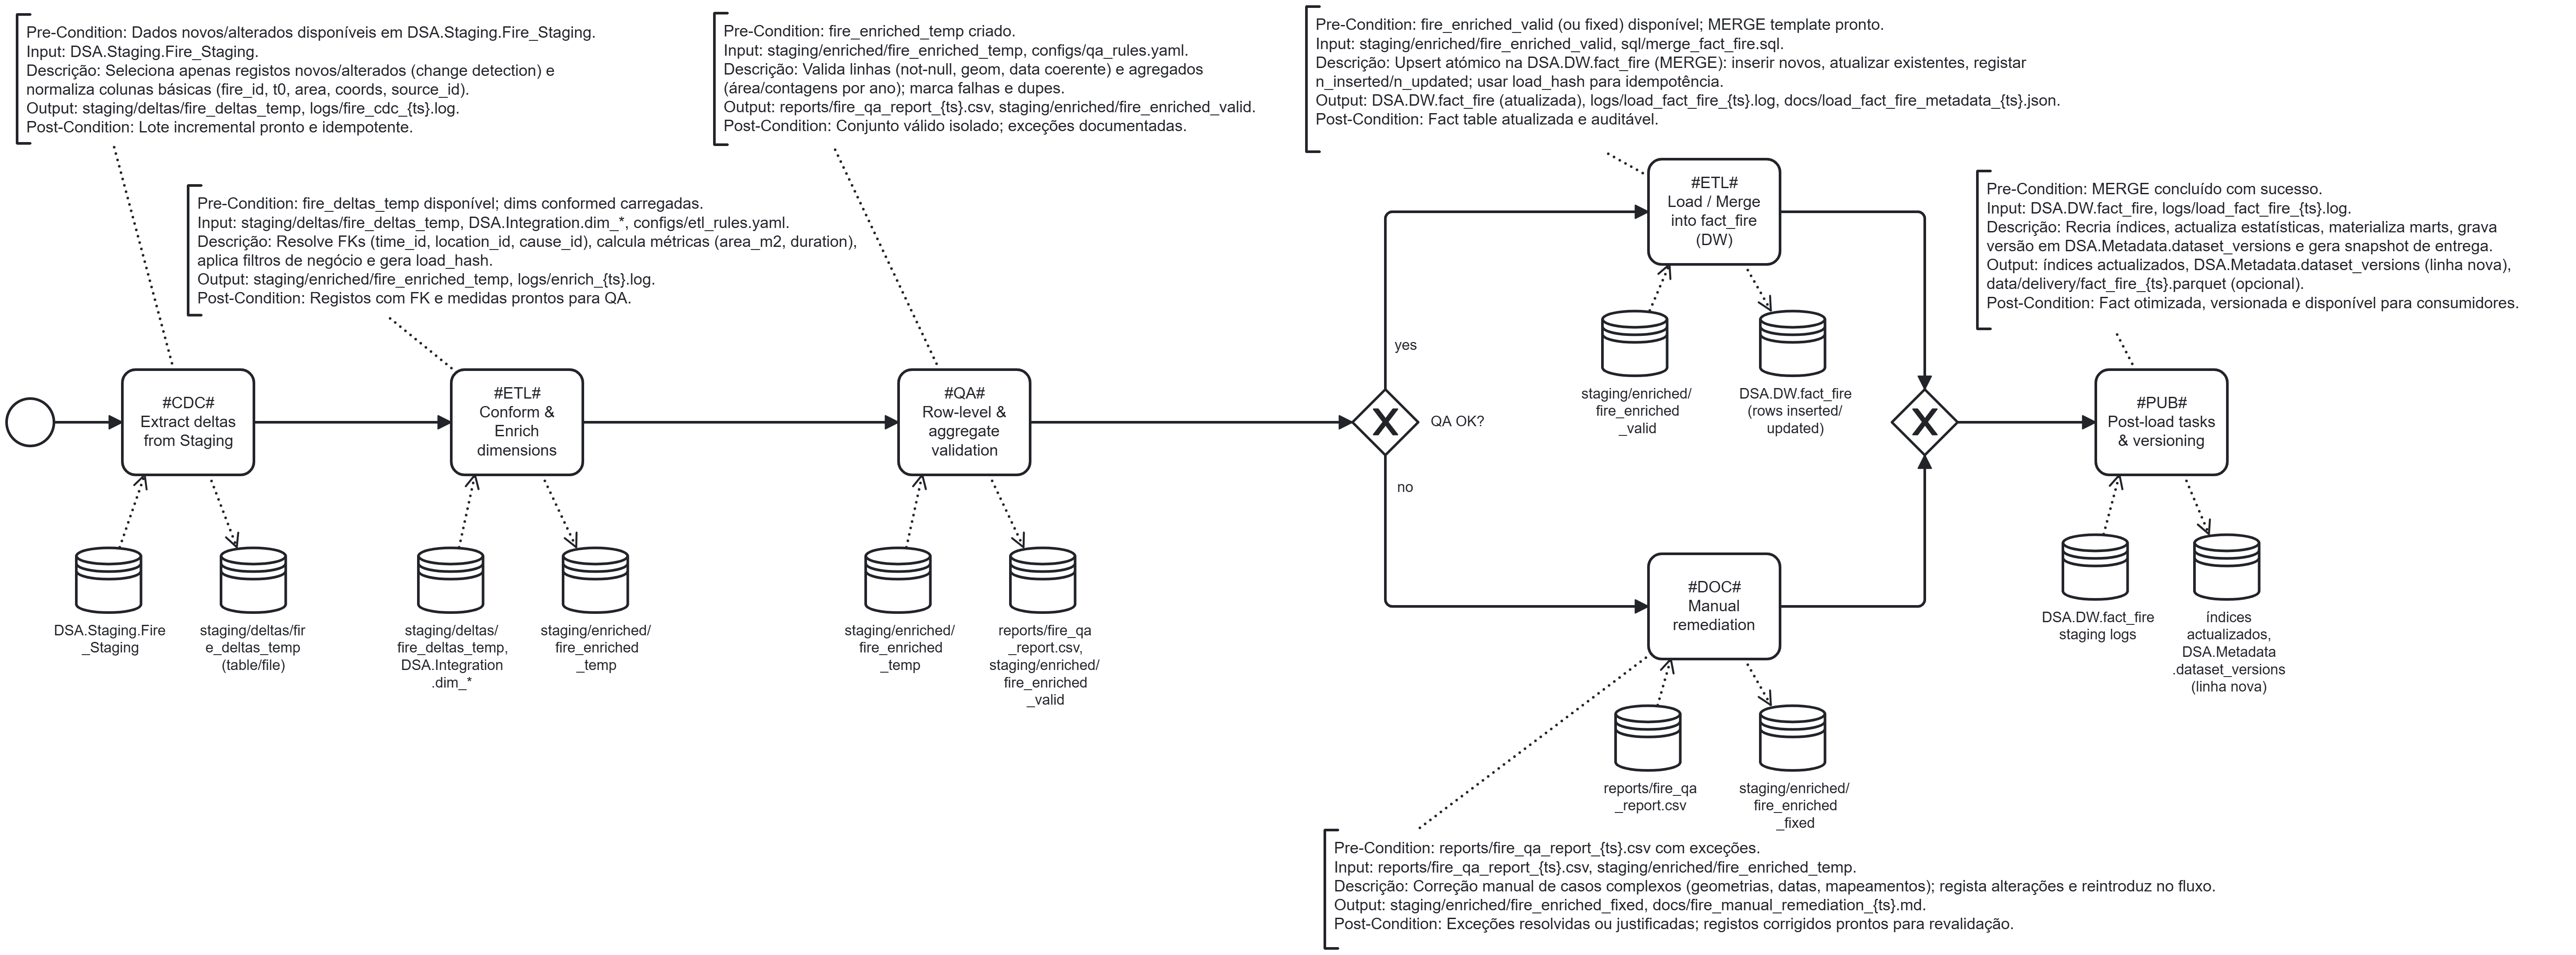
\includegraphics[width=1\linewidth]{imagens/BPMN_Processo_Load_Fire_Fact_Table}
	\caption{Diagrama BPMN nível padrão para tabela de factos de incêndio}
	\label{fig:bpmnprocessoloadfirefacttable}
\end{figure}

\begin{figure}[h]
	\centering
	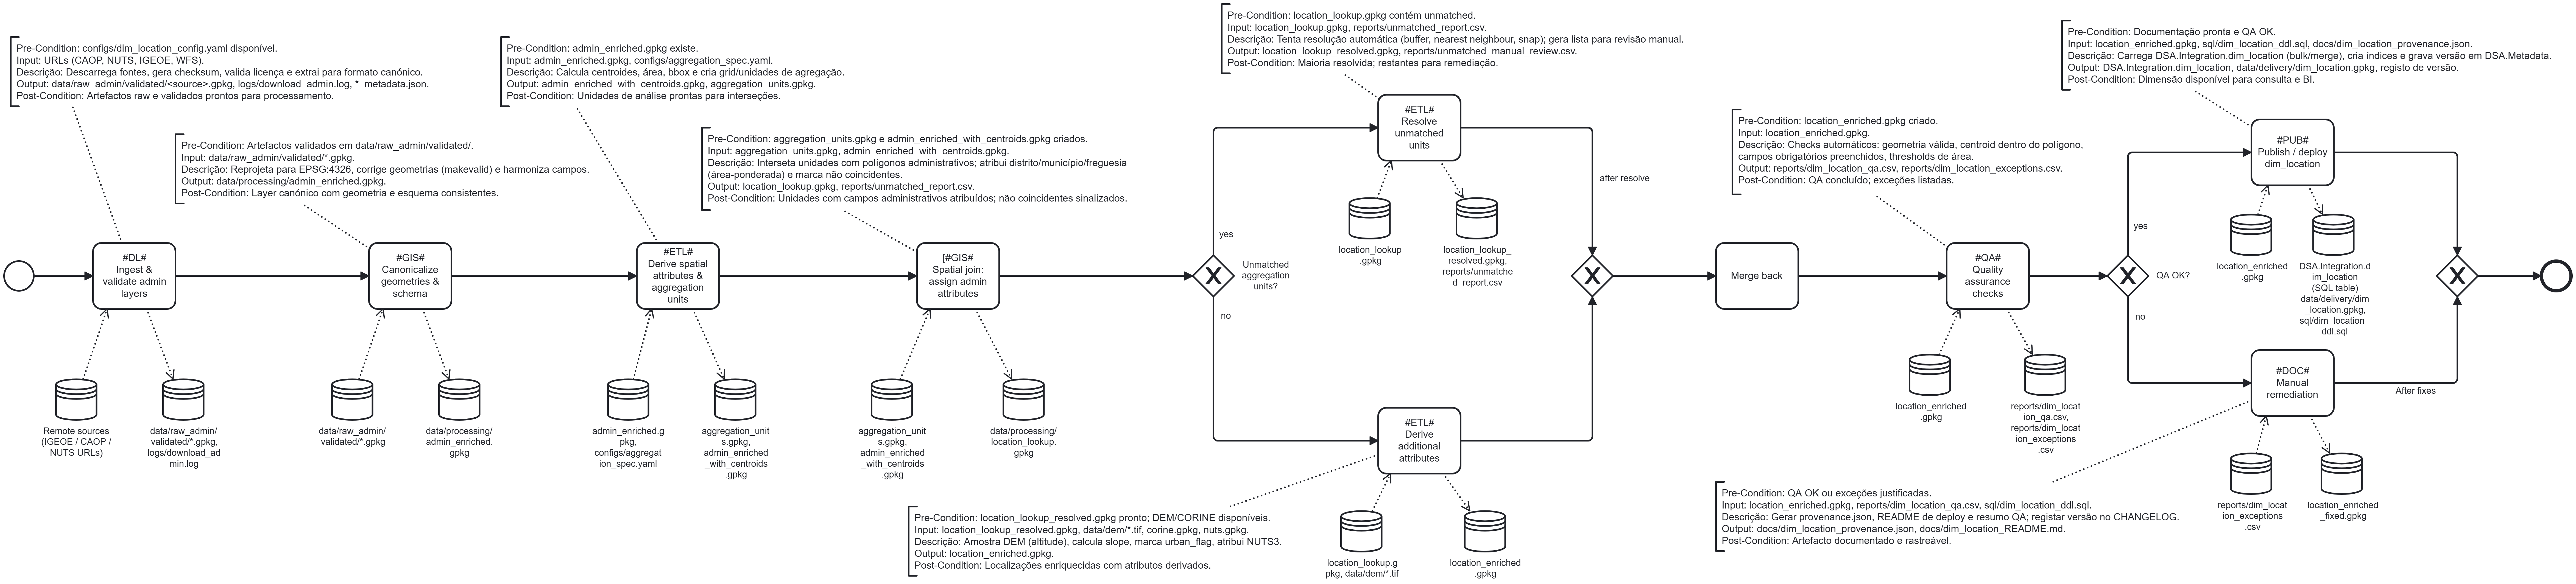
\includegraphics[width=1.2\linewidth]{imagens/BPMN_Processo_Load_Location_Dimension}
	\caption{Diagrama BPMN nível padrão para a dimensão de localização}
	\label{fig:bpmnprocessoloadlocationdimension}
\end{figure}



